\section{Moduł kompilujący}
W czasie prac nad projektem nie była dostępna istniejąca część systemu modułu kompilującego, odpowiedzialnego za kompilację kodu, wykonanie programu oraz przeprowadzanie testów. Znane były funkcjonalności oraz wymagania, które musiał spełniać ten moduł, co pozwoliło na implementację własnego modułu. Rozwiązanie w obecnym stanie było używane jedynie do testów, jednak jest otwarte na modyfikację i dalszy rozwój w przyszłości. W tym rozdziale zostanie opisany zaimplementowany przez nas moduł, a nie zintegrowany w ostatecznym rozwiązaniu kontener pochodzący z obecnego systemu STOS. Na etapie projektowania i implementacji nie był znany dokładny interfejs obrazu istniejącego kontenera, przez co nie jest on z nim kompatybilny. 

\subsection{Wymagania}
Otrzymane wymagania do modułu kompilującego obejmowały wykorzystane technologie oraz sposób działania. Moduł musiał być skonteneryzowany, zapewniając izolację wykonywanego kodu zadania od systemu operacyjnego i procesów systemu macierzystego. Ze względu na dostępność wiedzy, łatwość implementacji oraz utrzymywania systemu, oprogramowaniem służącym do konteneryzacji miał być Docker. Został również określony wymóg, aby czas wykonania zadania był niezależny od obciążenia i dostępnej mocy obliczeniowej systemu macierzystego. Dodatkowo system miał zapewniać wykonywanie programu zadania tak, jakby był wykonywany na maszynie z systemem operacyjnym Windows. Ważnym aspektem był również niski koszt związany z potencjalną awarią i ponownym przywróceniem działania tej części systemu.

\subsection{Obraz bazowy}
Wybranym obrazem bazowym do kontenera zostało Ubuntu 20.04 \cite{linuxUbuntu}, jest to popularny wybór, dzięki czemu jest dobrze przetestowany i kompatybilny z wieloma narzędziami. Obrazy Ubuntu dostępne w Docker Hub to systemy oparte na Ubuntu Base, czyli lżejszej wersji Ubuntu, nieposiadającej oprogramowania, które nie jest przydatne do pracy w kontenerze takich jak interfejs graficzny lub aplikacje biurowe. Wersja 20.04 jest wersją Long-Term Support, co oznacza, że przez długi czas oferuje aktualizacje bezpieczeństwa oraz poprawki. Posiada również bogate repozytorium pakietów, oferujące wszystkie potrzebne w naszym zastosowaniu narzędzia.

\subsection{Wykorzystane pakiety}
Wszystkie pakiety konieczne do prawidłowej pracy kontenera zostały pozyskane z repozytorium Ubuntu 20.04 przy pomocy systemu zarządzania pakietami apt-get. Obejmowały kompilator mingw, narzędzie Wine pozwalające na uruchamianie aplikacji przeznaczonych na system operacyjny Windows oraz wirtualny serwer Xvfb zapewniający wirtualne środowisko graficzne dla Wine.

\subsection{Wymiana plików między kontenerem a systemem macierzystym}
Narzędzie Docker zapewnia dwie podstawowe metody wymiany plików między kontenerem a systemem macierzystym - Docker Volume\cite{dockerVolume} oraz Bind mounts\cite{dockerBindMounts}. Docker Volume jest mechanizmem zarządzanym przez system Docker, odpowiada on za tworzenie, zarządzanie i usuwanie danych. Możliwe jest współdzielenie jednego wolumenu przez liczne kontenery. Bind mounts to prostsze rozwiązanie polegające na bezpośrednim połączeniu wybranego katalogu w systemie macierzystym z katalogiem kontenera. Zapewnia to większą elastyczność, ponieważ nie wymaga tworzenia osobnego wolumenu, a jedynie powiązania ścieżki bezwzględnej na systemie macierzystym, ze ścieżką wewnątrz kontenera, jednak tym samym zmniejsza to izolację kontenera od systemu. W naszym rozwiązaniu zostały wykorzystane bind mounts, ponieważ każde sprawdzane rozwiązanie otrzymuje swój osobny folder powiązany z jego id, który wiążemy z osobnym, nowo utworzonym kontenerem. Eliminuje to potrzebę zarządzania licznymi wolumenami lub dzielenia wolumenu między kilka kontenerów co z kolei zmniejszyłoby izolację między zadaniami. Aby zaimplementowany kontener poprawnie skompilował i uruchomił program, struktura powiązanego folderu powinna wyglądać w następujący sposób:
\begin{verbatim}
    /folder powiązany
    |-- /source
    |   |-- main.cpp
    |-- /input
    |   |-- 1.in
    |   |-- 2.in
    |   |-- n.in
    |-- /output
        |-- 1.out
        |-- 2.out
        |-- n.out
\end{verbatim}
W katalogu /source znajdują się pliki zawierające kod źródłowy c++. Wejście, które chcemy przekazać przy uruchamianiu programu, znajduje się w plikach *.in w folderze /input. W trakcie działania programu tworzone są pliki wynikowe z rozszerzeniem *.out w folderze /output. 

\subsection{Skrypt uruchamiany przy starcie kontenera}
Punkt wejścia to skrypt wskazany w pliku Dockerfile, który uruchamia się po starcie kontenera. Został napisany w Bashu i realizuje funkcjonalność modułu kompilującego, kompiluje pliki *.cpp znajdujące się w katalogu /source powiązanego folderu za pomocą mingw, a następnie uruchamia skompilowany program dla każdego z plików wejścia *.in umieszczonych w folderze /in. Wynik każdego uruchomienia przekierowywany jest do  pliku wynikowego *.out w folderze /out katalogu współdzielonego. Każde uruchomienie dodatkowo mierzy czas wykonania przy pomocy komendy date.
\begin{figure}[!ht]
	\begin{center}
		\resizebox{1\textwidth}{!} {
			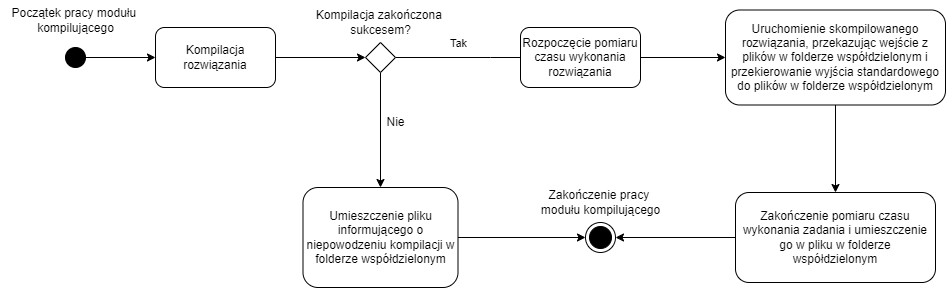
\includegraphics{img/3/diagram-aktywnosci-modul-kompilujacy.png}
		}
		\caption[Diagram aktywności modułu kompilującego]{Diagram wizualizujący przebieg pracy modułu kompilującego. Źródło własne.}
		\label{diagram-aktywnosci-worker}
	\end{center}
\end{figure}

\subsection{Ograniczenie zasobów kontenera}
Jednym z elementów zapewnienia sprawiedliwej oceny czasu wykonania zadania jest określenie maksymalnej ilości pamięci ram oraz zasobów procesora, które są dostępne dla kontenera. Domyślnie kontener nie posiada żadnych ograniczeń wykorzystywanych zasobów i wykorzystuje ich tyle, ile zostanie mu przydzielone przez jądro systemu macierzystego. Te wartości można jednak ograniczyć, korzystając z mechanizmu kontroli maksymalnych zasobów wykorzystanych przez kontener udostępnionego przez narzędzie Docker\cite{dockerConstraints}, poprzez użycie flag --memory oraz --cpus przy starcie kontenera. Zakładając, że przydzielone kontenerom zasoby nie przekraczają całości dostępnych zasobów komputera, możemy osiągnąć względnie sprawiedliwą ocenę czasu wykonania zadania. Rozwiązaniem, które pozwala z większą dokładnością określić zasoby czasowe potrzebne do wykonania programu, jest pomiar wykorzystania procesora na podstawie liczby cykli, jednak implementacja tej funkcjonalności wewnątrz kontenera dockerowego wiąże się z koniecznością uruchomienia go ze zwiększonymi uprawnieniami do funkcji jądra, co znacząco zmniejsza izolację modułu i bezpieczeństwo całego systemu, w szczególności biorąc pod uwagę fakt, że moduł ten odpowiada za kompilację i wykonanie potencjalnie szkodliwego kodu przesłanego przez użytkowników zewnętrznego systemu STOS.

\subsection{Różnice w funkcjonowaniu aplikacji na systemach Windows i Linux}
\subsubsection{Linux}
Systemy Linux to systemy bazujące jądrze Linux. Jądro to zostało udostępnione w 1991 przez Linusa Torvaldsa na licencji GNU General Public License, co oznacza, że jego kod źródłowy jest publicznie dostępny, a użytkownicy mają wolność do uruchamiania, analizowania, rozpowszechniania i udoskonalania programu.
Jest systemem uniksopodobnym i zgodny ze standardem POSIX, czyli jego monolityczna budowa jądra, model systemu plików, komunikacja międzyprocesowa, zarządzanie pamięcią, interfejs programistyczny i użytkownika są zbliżone do systemu Unix, jednak jego kod źródłowy nie wywodzi się z kodu źródłowego Uniksa. Struktura katalogów w systemie Linux jest zdefiniowana w Filesystem Hierarchy Standard \cite{linuxFhs} i składa się z katalogu głównego “/”, w którym znajdują się wszystkie inne katalogi, bazowo takie jak:
\begin{verbatim}
    /root
    |-- /bin/ - podstawowe pliki wykonynwalne (binaries)
    |-- /boot/ - pliki rozruchowe
    |-- /dev/ - pliki urządzeń
    |-- /etc/ - pliki konfiguracyjne
    |-- /tmp/ - pliki tymczasowe
    |-- /lib/ - biblioteki współdzielone
    |-- /var/ - pliki, których zawartość często ulega zmianie (np. logi)
    |-- /usr/ - pliki współdzielone i niezmienne
    |-- /home/ - pliki użytkownika
\end{verbatim}

\subsubsection{Windows}
Systemy Windows to systemy wyprodukowane przez firmę Microsoft, które od 1993 bazują na hybrydowym jądrze\cite{windowsHybridKernel} NT (New Technology)\cite{windowsNT} zawierające między innymi funkcje jak zarządzania procesami, pamięcią, urządzeniami, przerwaniami systemowymi, komunikacją między procesową. Hybrydowość jądra oznacza, że posiada ono jednocześnie cechy jądra monolitycznego oraz mikrojądra, w jądrze NT działa to na zasadzie przestrzeni jądra oraz przestrzeni użytkownika. Przestrzeń jądra posiada pełny dostęp do zarządzania pamięcią, procesami, systemem plików oraz urządzeń, a przestrzeń użytkownika to przestrzeń, w której te dostępy są ograniczone, a operacje dostępu do zasobów systemowych odbywają się, korzystając z interfejsu systemowego jądra, poprzez wołania systemowe. Taki podział ma na celu zwiększenie bezpieczeństwa i zmniejszenie podatności na awarię systemu. Domyślnym systemem plików w systemach bazujących na jądrze NT jest NTFS, w którym dyski rozdzielone są na partycje systemowe.

\subsubsection{Wpływ różnic na wykonanie aplikacji w obu systemach}
Różnice między systemem Linux a Windows są widoczne na każdym aspekcie, począwszy od jądra, systemu plików, wydajności, licencjonowania, dostępnego oprogramowania. Przekładają się na działanie aplikacji w tych systemach. Komunikacja programu z systemem operacyjnym jest oparta na innych, niekompatybilnych ze sobą interfejsach, oba systemy bazują na innych systemach plików. Aplikacje w systemie Windows korzystają z dynamicznie ładowanych systemowych bibliotek, a swoje ustawienia i konfiguracje często zapisują w rejestrze systemowym. Linuksowe odpowiedniki bibliotek .dll jako pliki .so oraz sposób zapisywania konfiguracji aplikacji w katalogu /etc/ nie są kompatybilne z Windowsem. Sprawia to, funkcjonowanie aplikacji, jak i proces kompilacji oraz wykonania kodu c++ różni się między dwoma systemami.

\subsection{Uruchamianie aplikacji przeznaczonych na system operacyjny Windows na systemie operacyjnym Linux}
\subsubsection{Emulator i warstwa kompatybilności}
Emulator to oprogramowanie tworzące wirtualną maszynę innej platformy. Uruchamianie aplikacji na emulatorze, nie różni się od uruchamiania jej na natywnej platformie, symulowany jest cały system docelowy. Wadą stosowania emulatora jest nieporównywalnie gorsza wydajność w porównaniu do natywnej platformy. W artykule\cite{emulatorPerformance} porównującym wydajność emulatorów Android Studio oraz Blue Stacks do urządzeń fizycznych z systemem Android, uzyskano od trzech, do nawet dwudziestu pięciu razy gorszą wydajność w aplikacji testowej polegającej na wykonaniu algorytmu szachowego mini-max. Warstwa kompatybilności również pozwala na uruchomienie aplikacji zaprojektowanej na inną platformę, jednak zamiast przeprowadzać kosztowną symulację całego systemu docelowego, zamienia ona wołania systemowe pochodzące z uruchamianego programu na te z systemu macierzystego, dzięki czemu aplikacja działa tak, jak działałaby na natywnej platformie, a system macierzysty otrzymuje właściwe dla siebie żądania. Dzięki braku konieczności symulowania całej maszyny warstwa kompatybilności zapewnia lepszą wydajność od emulatora i nie wymaga dużego nakładu pamięci.

\subsubsection{Wine\cite{wine}}
Wine to warstwa kompatybilności aplikacji przeznaczonych do wykonywania na systemie Windows na systemach zgodnych ze standardami POSIX, takich jak Linux, macOS. Jest oprogramowaniem open source, który jest wciąż aktywnie wspierany przez społeczność oraz firmę CodeWeavers, a jego pierwsza wersja został wydana w 1993 roku. Ze względu na to, że ponad 70\% komputerów osobistych korzysta z systemów operacyjnych Windows\cite{windowsMarketShare}, programy użytkowe takie jak aplikacje biznesowe, narzędzia biurowe czy gry komputerowe często tworzone są tylko na tę platformę, co może ograniczać użytkownikom możliwość wyboru używanego systemu, prowadzić do monopolu i wymuszać zakup licencji Windows. Wine oraz inne programy realizujące podobną funkcjonalność, pozwalają na wybór preferowanego systemu, bez rezygnowania z dostępu do puli programów nieoferujących wsparcia dla niego.

\begin{figure}[!h]
	\begin{center}
		\resizebox{1\textwidth}{!} {
			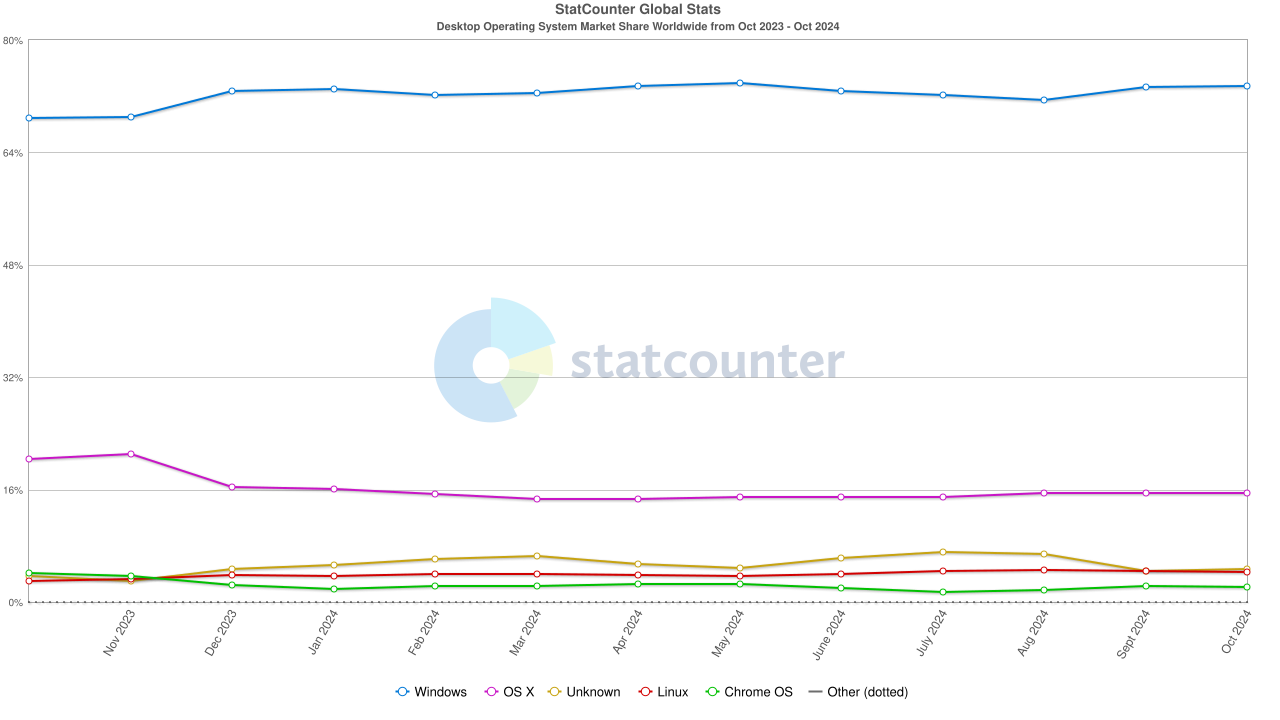
\includegraphics{img/3/desktop-os-market-share.png}
		}
		\caption{Wykres przedstawiający udział systemów operacyjnych wśród komputerów osobistych. Źródło: https://gs.statcounter.com/os-market-share/desktop/worldwide/.}
		\label{desktop-os-market-share}
	\end{center}
\end{figure}

Wine podczas pracy korzysta z folderu zawierającego wirtualne środowisko - Wineprefix\cite{wineprefix}, gdzie znajdują się pliki symulujące system Windows. Są tam pliki rejestrów, biblioteki, pliki konfiguracyjne oraz struktura folderów odpowiadająca podziałowi na partycje systemowe systemu Windows, które tworzone jest domyślne przy instalacji programu. Użytkownik może utworzyć więcej środowisk, z dostosowanymi ustawieniami architektury, narzędzi, bibliotek dll czy wersji systemu, oraz zmieniać wykorzystywane obecnie środowisko. Konfiguracja środowiska odbywa się przy pomocy narzędzia Winetricks\cite{winetricks}. Izoluje to działanie programu od wirtualnego środowiska i umożliwia konfigurację go do własnych potrzeb. Aby uruchomić program przy pomocy Wine, należy uruchomić go za pomocą komendy:
\begin{verbatim}
wine <plik wykonywalny>
\end{verbatim} Wine ładuje program do pamięci, parsuje go, dołącza potrzebne zależności i przechodzi do wykonywania programu. Gdy w trakcie pracy programu pojawi się wołanie systemowe, Wine przechwytuje je i zamienia na zgodne ze standardami POSIX. 

Wine jako projekt otwartoźródłowy jest bazą licznych alternatyw\cite{wineBasedProjects} z których najbardziej zaawansowanymi są Proton\cite{proton} oraz CrossOver\cite{crossover}. CrossOver to płatne oprogramowanie firmy CodeWeavers, czyli firmy, która również zajmuje się rozwojem projektu Wine. W odróżnieniu od Wine, CrossOver zapewenia graficzny interfejs użytkownika. Dodatkowo, rozwój Wine jest bardziej restrykcyjny i czasochłonny - nowe funkcjonalności muszą zostać zaimplementowane w sposób zgodny z określonymi standardami, tak, aby tłumaczenie wołań systemowych odbywało się w jak najbardziej dokładny sposób. W przypadku CrossOver rozwój stawia bardziej na aspekty użytkowe - w celu szybszego naprawienia problemu występującego w aplikacji często używanej przez użytkowników programu, twórcy mogą wprowadzić zmiany specyficzne dla danej aplikacji, aby ten konkretny problem nie występował. Z czasem może to zostać naprawione w sposób należyty w wersji Wine, które to są regularnie integrowane do kodu źródłowego CrossOver.

Proton opracowywany jest przez Valve, realizuje podobną funkcjonalność, jednak jego rozwój jest skupiony na zapewnieniu poprawnego działania platformy Steam oraz gier przeznaczonych na tę platformę w systemie Linux poprzez warstwę kompatybilności między programistycznym interfejsem przeznaczonym na systemy Windows - Direct3D, służącym do rysowania trójwymiarowych obiektów, na wieloplatformowy odpowiednik - Vulkan.

